\section{Motivation and Scope}

There has been a strong desire for a more space- and/or runtime-efficient
representation for \code{map} among C++ users for some time now.  This has
motivated discussions among the members of SG14 resulting in a
paper\footnote{See P0038R0,
  \href{http://www.open-std.org/jtc1/sc22/wg21/docs/papers/2015/p0038r0.html}{here}.},
numerous articles and talks, and an implementation in Boost,
\code{boost::container::flat_map}\footnote{Part of Boost.Container,
  \href{http://www.boost.org/doc/libs/1_61_0/doc/html/container.html}{here}.}.
Virtually everyone who makes games, embedded, or system software in C++ uses
the Boost implementation or one that they rolled themselves.\\

Here are some numbers that show why.  The graphs that follow show runtimes for
different \code{map}-like associative containers.  The containers used are
Boost.FlatMap, \code{map}, and two thin wrappers over a sorted \code{vector};
the ``custom pair'' version of the sorted \code{vector} uses a simple
\code{struct} instead of \code{pair} for its value type.  All containers use
an \code{int} as the key type and an \code{int} or a \code{struct} with 5
\code{double}s for the value type.\\

All the graphs below were produced on Windows with MSVC 2015.  Similar results
were obtained on Linux, with Clang 3.9 and libc++, and with g++ 4.8.4 and
libstdc++.\\

These first four graphs cover the \code{int}-value-type case.  The first graph
shows insertion of N elements with random keys; the second shows full
iteration across all N elements; the third shows \code{map.lower_bound()}
called once for each key used in the original insertions; and the fourth shows
erasure of all N elements, by the keys used in the original insertions.

\begin{center}
    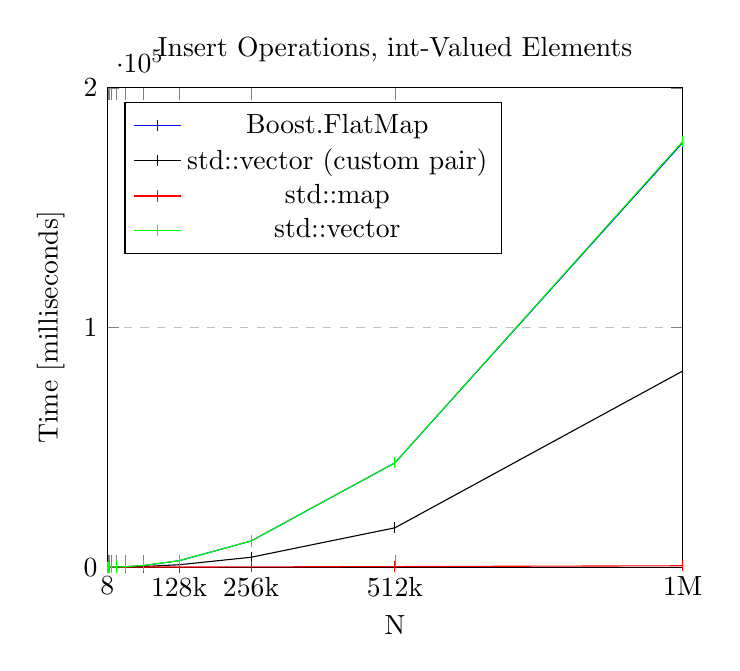
\begin{tikzpicture}
    \begin{axis}[
        width=3.5in,
        title={Insert Operations, int-Valued Elements},
        xlabel={N},
        ylabel={Time [milliseconds]},
        xmin=0, xmax=1048576,
        ymin=0, ymax=200000.0,
        xtick={8,16,32,64,128,256,512,1024,2048,4096,8192,16384,32768,65536,131072,262144,524288,1048576,2097152},
        xticklabels={8,,,,,,,,,,,,,,128k,256k,512k,1M,2M},
        ytick={0.0,100000.0,200000.0,300000.0},
        legend pos=north west,
        ymajorgrids=true,
        grid style=dashed,
        scaled x ticks=false,
        scaled y ticks=true,
        legend entries={Boost.FlatMap,std::vector (custom pair),std::map,std::vector},
        ]

    \addplot[color=blue,mark=|,]
        coordinates {(8,0.000781)(16,0.0015024)(32,0.002704)(64,0.0126796)(128,0.0220544)(256,0.0434464)(512,0.0975326)(1024,0.243922)(2048,0.996534)(4096,2.74574)(8192,10.778)(16384,39.5847)(32768,151.266)(65536,645.843)(131072,2656.72)(262144,10886.4)(524288,43508.8)(1048576,177152)};

    \addplot[color=black,mark=|,]
        coordinates {(8,0.000901)(16,0.0019236)(32,0.003425)(64,0.0069706)(128,0.0185096)(256,0.0302876)(512,0.0681476)(1024,0.150657)(2048,0.381718)(4096,1.13392)(8192,3.84725)(16384,14.6989)(32768,56.4104)(65536,233.755)(131072,977.843)(262144,4108.92)(524288,16395.8)(1048576,81818.6)};

    \addplot[color=red,mark=|,]
        coordinates {(8,0.0009616)(16,0.0025234)(32,0.0048074)(64,0.0094356)(128,0.0223544)(256,0.0387004)(512,0.0793824)(1024,0.252635)(2048,0.361766)(4096,0.722497)(8192,1.55871)(16384,3.58995)(32768,7.77012)(65536,17.2662)(131072,37.8691)(262144,83.3477)(524288,216.148)(1048576,554.857)};

    \addplot[color=green,mark=|,]
        coordinates {(8,0.000841)(16,0.0017426)(32,0.003606)(64,0.0073914)(128,0.016226)(256,0.034913)(512,0.0902026)(1024,0.301429)(2048,0.783507)(4096,2.80837)(8192,10.8466)(16384,40.9552)(32768,168.836)(65536,664.013)(131072,2694.41)(262144,10889.2)(524288,43577.6)(1048576,177594)};

    \end{axis}
\end{tikzpicture}
\end{center}


As one might expect, insertionion takes longer in contiguous-storage
implementations.  Boost.FlatMap and a sorted \code{vector<pair<int, int>>}
have superlinear growth in insertion time.  While the curve for sorted
\code{vector} using a custom \code{struct} instead of a \code{pair} is
superlinear as well, it is dramatically flatter in its growth -- much closer
to node-based \code{map}.

\begin{center}
    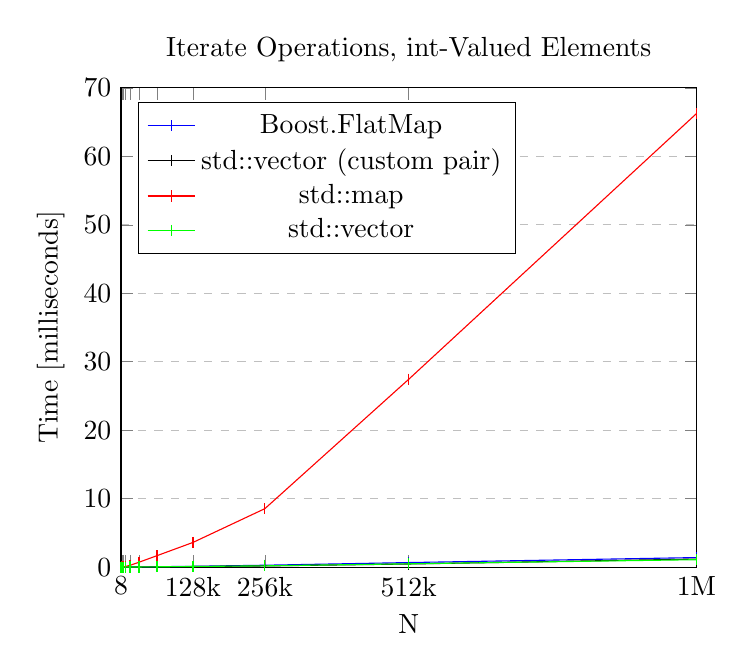
\begin{tikzpicture}
    \begin{axis}[
        width=3.5in,
        title={Iterate Operations, int-Valued Elements},
        xlabel={N},
        ylabel={Time [milliseconds]},
        xmin=0, xmax=1048576,
        ymin=0, ymax=70.0,
        xtick={8,16,32,64,128,256,512,1024,2048,4096,8192,16384,32768,65536,131072,262144,524288,1048576,2097152},
        xticklabels={8,,,,,,,,,,,,,,128k,256k,512k,1M,2M},
        ytick={0.0,10.0,20.0,30.0,40.0,50.0,60.0,70.0,80.0},
        legend pos=north west,
        ymajorgrids=true,
        grid style=dashed,
        scaled x ticks=false,
        scaled y ticks=true,
        legend entries={Boost.FlatMap,std::vector (custom pair),std::map,std::vector},
        ]

    \addplot[color=blue,mark=|,]
        coordinates {(8,0.00012)(16,6e-05)(32,0)(64,0.00024)(128,0.0001802)(256,0.0002404)(512,0.0003604)(1024,0.000661)(2048,0.001502)(4096,0.0030044)(8192,0.0066702)(16384,0.0126202)(32768,0.0245182)(65536,0.0533636)(131072,0.115741)(262144,0.272226)(524288,0.660912)(1048576,1.39117)};

    \addplot[color=black,mark=|,]
        coordinates {(8,0)(16,6e-05)(32,0)(64,6e-05)(128,0.00012)(256,0)(512,0.0003006)(1024,0.0003006)(2048,0.0007814)(4096,0.0015026)(8192,0.003185)(16384,0.0073918)(32768,0.0163456)(65536,0.0379792)(131072,0.0802854)(262144,0.17277)(524288,0.453048)(1048576,1.17087)};

    \addplot[color=red,mark=|,]
        coordinates {(8,6e-05)(16,0.0001202)(32,0.0002406)(64,0.0004208)(128,0.0010816)(256,0.0016828)(512,0.003185)(1024,0.0158046)(2048,0.0183286)(4096,0.0433276)(8192,0.0959696)(16384,0.253837)(32768,0.709108)(65536,1.66767)(131072,3.60046)(262144,8.53718)(524288,27.4399)(1048576,66.2461)};

    \addplot[color=green,mark=|,]
        coordinates {(8,0)(16,0)(32,0.00012)(64,6e-05)(128,6e-05)(256,0)(512,0.0002404)(1024,0.0003004)(2048,0.0007214)(4096,0.0017428)(8192,0.0042664)(16384,0.008413)(32768,0.0177278)(65536,0.0395418)(131072,0.0892992)(262144,0.182866)(524288,0.479309)(1048576,1.08127)};

    \end{axis}
\end{tikzpicture}
\end{center}


For all variants but \code{map}, iteration is relatively similar, and much
faster that \code{map}'s.

\begin{center}
    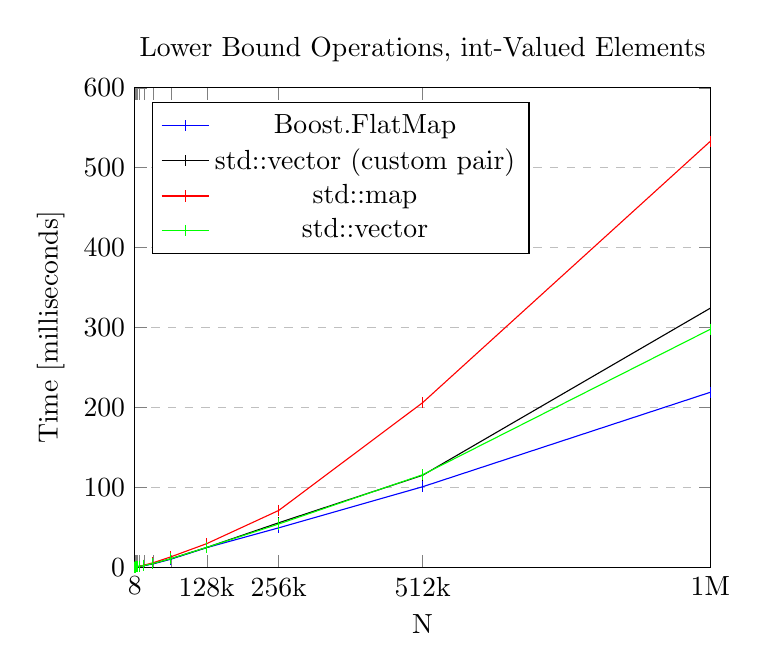
\begin{tikzpicture}
    \begin{axis}[
        width=3.5in,
        title={Lower Bound Operations, int-Valued Elements},
        xlabel={N},
        ylabel={Time [milliseconds]},
        xmin=0, xmax=1048576,
        ymin=0, ymax=600.0,
        xtick={8,16,32,64,128,256,512,1024,2048,4096,8192,16384,32768,65536,131072,262144,524288,1048576,2097152},
        xticklabels={8,,,,,,,,,,,,,,128k,256k,512k,1M,2M},
        ytick={0.0,100.0,200.0,300.0,400.0,500.0,600.0,700.0},
        legend pos=north west,
        ymajorgrids=true,
        grid style=dashed,
        scaled x ticks=false,
        scaled y ticks=true,
        legend entries={Boost.FlatMap,std::vector (custom pair),std::map,std::vector},
        ]

    \addplot[color=blue,mark=|,]
        coordinates {(8,0.0005406)(16,0.0008412)(32,0.0019234)(64,0.0053474)(128,0.0093136)(256,0.0221146)(512,0.0426054)(1024,0.0911624)(2048,0.187127)(4096,0.401311)(8192,0.92868)(16384,1.79835)(32768,3.93068)(65536,9.84609)(131072,24.3821)(262144,49.1404)(524288,100.579)(1048576,218.895)};

    \addplot[color=black,mark=|,]
        coordinates {(8,0.000541)(16,0.0010818)(32,0.0028844)(64,0.004627)(128,0.0113584)(256,0.0228948)(512,0.0471132)(1024,0.0959108)(2048,0.197415)(4096,0.437544)(8192,0.94612)(16384,2.01002)(32768,4.33019)(65536,10.4976)(131072,24.5992)(262144,55.4928)(524288,114.931)(1048576,324.188)};

    \addplot[color=red,mark=|,]
        coordinates {(8,0.0003606)(16,0.000962)(32,0.0018036)(64,0.003366)(128,0.0113572)(256,0.0203114)(512,0.0421244)(1024,0.108408)(2048,0.194106)(4096,0.422878)(8192,0.95153)(16384,2.36638)(32768,5.34999)(65536,12.8311)(131072,29.3991)(262144,70.921)(524288,205.833)(1048576,533.131)};

    \addplot[color=green,mark=|,]
        coordinates {(8,0.0004206)(16,0.0010822)(32,0.0025242)(64,0.0048678)(128,0.0102766)(256,0.0227732)(512,0.0474772)(1024,0.093809)(2048,0.194044)(4096,0.419156)(8192,0.937409)(16384,1.91502)(32768,4.41762)(65536,10.4906)(131072,24.6681)(262144,53.9334)(524288,115.602)(1048576,297.785)};

    \end{axis}
\end{tikzpicture}
\end{center}


\code{lower_bound()} performance is roughly similar across all the
implementations, and they all show superlinear growth.  Note that
Boost.FlatMap performs the best here.

\begin{center}
    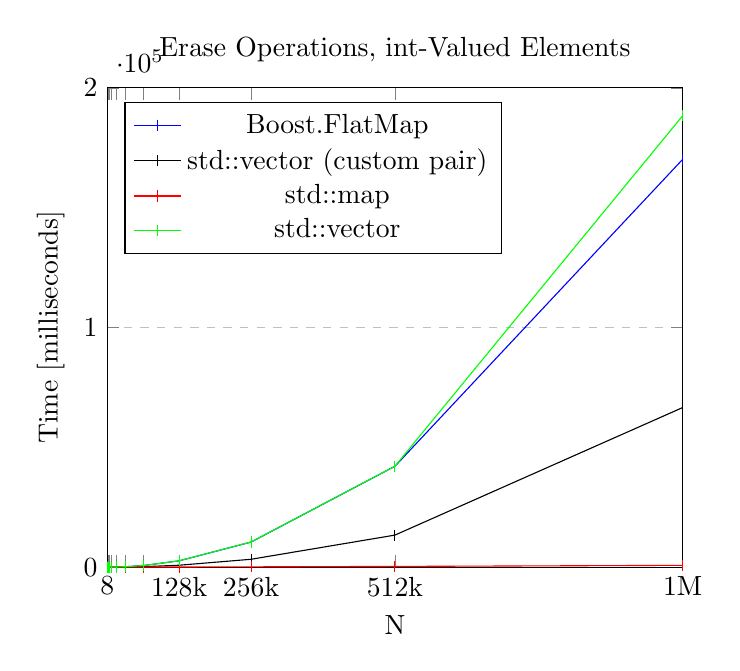
\begin{tikzpicture}
    \begin{axis}[
        width=3.5in,
        title={Erase Operations, int-Valued Elements},
        xlabel={N},
        ylabel={Time [milliseconds]},
        xmin=0, xmax=1048576,
        ymin=0, ymax=200000.0,
        xtick={8,16,32,64,128,256,512,1024,2048,4096,8192,16384,32768,65536,131072,262144,524288,1048576,2097152},
        xticklabels={8,,,,,,,,,,,,,,128k,256k,512k,1M,2M},
        ytick={0.0,100000.0,200000.0,300000.0},
        legend pos=north west,
        ymajorgrids=true,
        grid style=dashed,
        scaled x ticks=false,
        scaled y ticks=true,
        legend entries={Boost.FlatMap,std::vector (custom pair),std::map,std::vector},
        ]

    \addplot[color=blue,mark=|,]
        coordinates {(8,0.0006008)(16,0.0012012)(32,0.0022238)(64,0.0054076)(128,0.0123804)(256,0.031067)(512,0.0803454)(1024,0.270482)(2048,0.749789)(4096,2.59431)(8192,10.3877)(16384,38.589)(32768,152.922)(65536,634.029)(131072,2623.4)(262144,10439.8)(524288,42082.3)(1048576,170172)};

    \addplot[color=black,mark=|,]
        coordinates {(8,0.0004206)(16,0.0009008)(32,0.0020434)(64,0.0045672)(128,0.0115388)(256,0.0233782)(512,0.0510192)(1024,0.117966)(2048,0.285149)(4096,0.831815)(8192,2.82244)(16384,10.3968)(32768,39.7867)(65536,170.698)(131072,781.175)(262144,3265.41)(524288,13351)(1048576,66586.9)};

    \addplot[color=red,mark=|,]
        coordinates {(8,0.0007214)(16,0.002404)(32,0.0036658)(64,0.0070908)(128,0.0231958)(256,0.0356962)(512,0.0817874)(1024,0.188813)(2048,0.399261)(4096,0.981397)(8192,1.83544)(16384,4.25969)(32768,9.1862)(65536,21.7346)(131072,47.8383)(262144,107.716)(524288,281.668)(1048576,731.531)};

    \addplot[color=green,mark=|,]
        coordinates {(8,0.0004806)(16,0.0009614)(32,0.0017422)(64,0.004567)(128,0.013521)(256,0.0300466)(512,0.0794428)(1024,0.233224)(2048,0.79781)(4096,2.66654)(8192,10.272)(16384,39.5269)(32768,159.483)(65536,638.256)(131072,2611.55)(262144,10479.7)(524288,42101)(1048576,188357)};

    \end{axis}
\end{tikzpicture}
\end{center}


Erasure has a similar performance profile to insertion, except that the sorted
\code{vector<pair<int, int>>} performs substantially better than
Boost.FlatMap.\\


\subsection{Implications}

TODO Iteration is vastly cheaper for contiguous-storage variants.  It has been
suggested that a \code{map} with a custom allocator can achieve similar
performance to flat data structures, but this would not apply to iteration
performance, unless the values were added to the \code{map} in sorted order.\\

In all the graphs above, the reason the custom-\code{pair} sorted vector
performs so much better than \code{vector<pair<int, int>>} seems to be that
the custom-\code{pair} type has \code{nothrow} special functions.
Implementing all the special functions and adding \code{nothrow(false)} to
each makes the custom-\code{pair} version perform identically to the
\code{pair<int, int>} version.

Boost.FlatMap differs quite a bit from a sorted \code{vector}.  Clearly there
are a lot of QOI choices to make in implementing a standard \code{flat_map}.
